% Calculating the NOE.
%%%%%%%%%%%%%%%%%%%%%%

\chapter{Calculating the NOE} \label{ch: NOE}
\index{NOE|textbf}


\begin{figure*}[h]
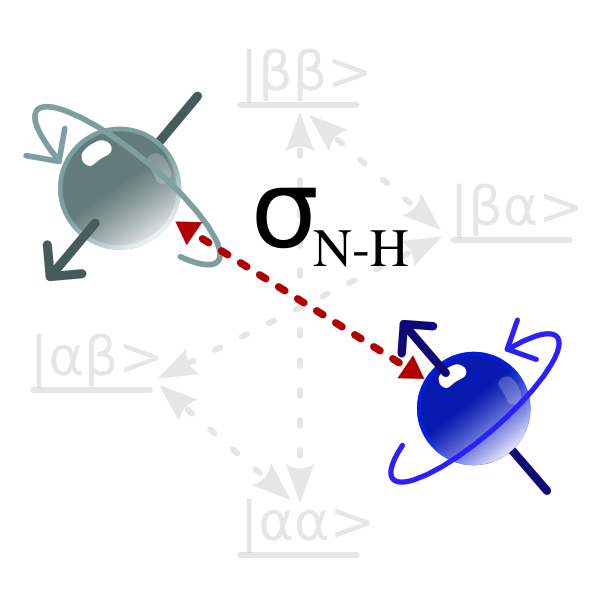
\includegraphics[width=5cm, bb=0 0 1701 1701]{graphics/analyses/noe_600x600}
\end{figure*}


% Introduction.
%%%%%%%%%%%%%%%

\section{Introduction to the steady-state NOE}

The calculation of NOE values is a straight forward and quick procedure which involves two components -- the calculation of the value itself and the calculation of the errors.  To understand the steps involved the execution of a sample NOE calculation script will be followed in detail.  Then the same operations will be presented for the perspective of the graphical user interface.



% From spectra to peak intensities.
%%%%%%%%%%%%%%%%%%%%%%%%%%%%%%%%%%%

\section{From spectra to peak intensities for the NOE}

For a set of recommendations for how to obtain the best quality relaxation rates, please see section~\ref{sect: spectra to intensities} on page~\pageref{sect: spectra to intensities}.  In summary the following are important -- temperature control (though the standard steady-state NOE single FID interleaved pulse sequences are fine), per-experiment temperature calibration, spectral processing with massive zero-filling and no baseplane rolling, and using an averaged peak list for determining the peak heights.



% Script UI.
%%%%%%%%%%%%

\section{Calculation of the NOE in the prompt/script UI mode}


% The sample script.
%~~~~~~~~~~~~~~~~~~~

\subsection{NOE script mode -- the sample script}

This sample script can be found in the \directory{sample\_scripts} directory and will be used as the template for the next sections describing how to use relax.

\begin{lstlisting}
# Script for calculating NOEs.

# Create the data pipe.
pipe.create('NOE', 'noe')

# Load the sequence from a PDB file.
structure.read_pdb('Ap4Aase_new_3.pdb')
structure.load_spins(spin_id='@N')
structure.load_spins(spin_id='@NE1')

# Load the reference spectrum and saturated spectrum peak intensities.
spectrum.read_intensities(file='ref.list', spectrum_id='ref_ave', heteronuc='N', proton='HN')
spectrum.read_intensities(file='ref.list', spectrum_id='ref_ave', heteronuc='NE1', proton='HE1')
spectrum.read_intensities(file='sat.list', spectrum_id='sat_ave', heteronuc='N', proton='HN')
spectrum.read_intensities(file='sat.list', spectrum_id='sat_ave', heteronuc='NE1', proton='HE1')

# Set the spectrum types.
noe.spectrum_type('ref', 'ref_ave')
noe.spectrum_type('sat', 'sat_ave')

# Set the errors.
spectrum.baseplane_rmsd(error=3600, spectrum_id='ref_ave')
spectrum.baseplane_rmsd(error=3000, spectrum_id='sat_ave')

# Individual residue errors.
spectrum.baseplane_rmsd(error=122000, spectrum_type='ref', res_num=114)
spectrum.baseplane_rmsd(error=8500, spectrum_type='sat', res_num=114)

# Peak intensity error analysis.
spectrum.error_analysis()

# Deselect unresolved residues.
deselect.read(file='unresolved', res_num_col=1, spin_name_col=2)

# Calculate the NOEs.
calc()

# Save the NOEs.
value.write(param='noe', file='noe.out', force=True)

# Create grace files.
grace.write(y_data_type='ref', file='ref.agr', force=True)
grace.write(y_data_type='sat', file='sat.agr', force=True)
grace.write(y_data_type='noe', file='noe.agr', force=True)

# View the grace files.
grace.view(file='ref.agr')
grace.view(file='sat.agr')
grace.view(file='noe.agr')

# Write the results.
results.write(file='results', dir=None, force=True)

# Save the program state.
state.save('save', force=True)
\end{lstlisting}



% Initialisation of the data pipe.
%~~~~~~~~~~~~~~~~~~~~~~~~~~~~~~~~~

\subsection{NOE script mode -- initialisation of the data pipe} \label{NOE initialisation}

The start of this sample script is very similar to that of the relaxation curve-fitting calculation on page~\pageref{Rx initialisation}.  The command

\begin{lstlisting}
pipe.create('NOE', 'noe')
\end{lstlisting}

initialises the data pipe labelled \promptstring{NOE}.  The data pipe type is set to the NOE calculation by the argument \promptstring{noe}.


% Spin systems.
%~~~~~~~~~~~~~~

\subsection{NOE script mode -- setting up the spin systems}

The backbone amide nitrogen sequence is extracted from a PDB\index{PDB} file using the same commands as the relaxation curve-fitting script (Chapter~\ref{ch: relax-fit}.  The command

\begin{lstlisting}
structure.read_pdb('Ap4Aase_new_3.pdb')
\end{lstlisting}
\index{PDB}

will load the PDB file \file{Ap4Aase\_new\_3.pdb} into relax.  Then the following commands will generate both the backbone amide and tryptophan indole $^{15}$N spins

\begin{lstlisting}
structure.load_spins(spin_id='@N')
structure.load_spins(spin_id='@NE1')
\end{lstlisting}


% Loading the data.
%~~~~~~~~~~~~~~~~~~

\subsection{NOE script mode -- loading the data}

The commands

\begin{lstlisting}
spectrum.read_intensities(file='ref.list', spectrum_id='ref_ave', heteronuc='N', proton='HN')
spectrum.read_intensities(file='ref.list', spectrum_id='ref_ave', heteronuc='NE1', proton='HE1')
spectrum.read_intensities(file='sat.list', spectrum_id='sat_ave', heteronuc='N', proton='HN')
spectrum.read_intensities(file='sat.list', spectrum_id='sat_ave', heteronuc='NE1', proton='HE1')
\end{lstlisting}

will load the peak heights\index{peak!height} of the reference and saturated NOE experiments (although the volume\index{peak!volume} could be used instead).  relax will automatically determine the format of the peak list.  Currently only Sparky\index{software!Sparky}, XEasy\index{software!XEasy}, NMRView\index{software!NMRView} and a generic columnar formatted text file are supported.

In this example, relax will determine from the file contents that these are Sparky\index{software!Sparky} peak lists (saved after typing \gui{lt}).  The first column of the file should be the Sparky assignment string and it is assumed that the 4$^\textrm{th}$ column contains either the peak height or peak volume (though this can be in any column -- the \prompt{int\_col} argument is used to specify where the data is).  Without specifying the \prompt{int\_method} argument, peak heights will be assumed.  See page~\pageref{uf: spectrum.read_intensities} for a description of all the \uf{spectrum.read\_intensities} user function arguments.  In this example, the peak list looks like:

{\footnotesize \begin{verbatim}
     Assignment         w1         w2   Data Height

        LEU3N-HN    122.454      8.397       129722
        GLY4N-HN    111.999      8.719       422375
        SER5N-HN    115.085      8.176       384180
        MET6N-HN    120.934      8.812       272100
        ASP7N-HN    122.394      8.750       174970
        SER8N-HN    113.916      7.836       218762
       GLU11N-HN    122.194      8.604        30412
       GLY12N-HN    110.525      9.028        90144
\end{verbatim}}

For subsequent usage of the data in relax, assuming a 3D structure exists, it is currently advisable to use the same residue and atom numbering as found in the PDB file.

If you have any other format you would like read by relax please send an email to the relax development mailing list\index{mailing list!relax-devel} detailing the software used, the format of the file (specifically where the residue number and peak intensity\index{peak!intensity} are located), and possibly attaching an example of the file itself.



% Setting the errors.
%~~~~~~~~~~~~~~~~~~~~

\subsection{NOE script mode -- setting the errors}

In this example the errors where measured from the base plain noise.  The Sparky\index{software!Sparky} RMSD\index{RMSD} function was used to estimate the maximal noise levels across the spectrum in regions containing no peaks.  For the reference spectrum the RMSD was approximately 3600 whereas in the saturated spectrum the RMSD was 3000.  These errors are set by the commands

\begin{lstlisting}
spectrum.baseplane_rmsd(error=3600, spectrum_id='ref_ave')
spectrum.baseplane_rmsd(error=3000, spectrum_id='sat_ave')
\end{lstlisting}

For the residue G114, the noise levels are significantly increased compared to the rest of the protein as the peak is located close to the water signal.  The higher errors for this residue are specified by the commands

\begin{lstlisting}
spectrum.baseplane_rmsd(error=122000, spectrum_type='ref', res_num=114)
spectrum.baseplane_rmsd(error=8500, spectrum_type='sat', res_num=114)
\end{lstlisting}

There are many other ways of setting the errors, for example via spectrum duplication, triplication, etc.  See the documentation for the \uf{spectrum.error\_analysis} user function on page~\pageref{uf: spectrum.error_analysis} for all possible options.  This user function needs to be executed at this stage to correctly set up the errors for all spin systems:

\begin{lstlisting}
spectrum.error_analysis()
\end{lstlisting}


% Unresolved spins.
%~~~~~~~~~~~~~~~~~~

\subsection{NOE script mode -- unresolved spins}

As the peaks of certain spins overlap to such an extent that the heights or volumes cannot be resolved, a simple text file was created called \promptstring{unresolved} in which each line consists of the residue number followed by the atom name.  By using the command

\begin{lstlisting}
deselect.read(name, file='unresolved', res_num_col=1, spin_name_col=2)
\end{lstlisting}

all spins in the file \promptstring{unresolved} are excluded from the analysis.



% The NOE.
%~~~~~~~~~

\subsection{NOE script mode -- the NOE calculation}

At this point the NOE can be calculated.  The user function

\begin{lstlisting}
calc()
\end{lstlisting}

will calculate both the NOE and the errors.  The NOE value will be calculated using the formula
\begin{equation}
NOE = \frac{I_{sat}}{I_{ref}},
\end{equation}

\noindent where $I_{sat}$ is the intensity of the peak in the saturated spectrum and $I_{ref}$ is that of the reference spectrum.  The error is calculated by
\begin{equation}
\sigma_{NOE} = \sqrt{\frac{(\sigma_{sat} \cdot I_{ref})^2 + (\sigma_{ref} \cdot I_{sat})^2}{I_{ref}}},
\end{equation}

\noindent where $\sigma_{sat}$ and $\sigma_{ref}$ are the peak intensity errors in the saturated and reference spectra respectively.  To create a file of the NOEs the command

\begin{lstlisting}
value.write(param='noe', file='noe.out', force=True)
\end{lstlisting}

will create a file called \file{noe.out} with the NOE values and errors.  The force flag will cause any file with the same name to be overwritten.  An example of the format of \file{noe.out} is

{\scriptsize \begin{verbatim}
# mol_name          res_num  res_name  spin_num  spin_name  value                  error                   
Ap4Aase_new_3_mol1  1        GLY       1         N          None                   None                    
Ap4Aase_new_3_mol1  2        PRO       11        N          None                   None                    
Ap4Aase_new_3_mol1  3        LEU       28        N          None                   None                    
Ap4Aase_new_3_mol1  4        GLY       51        N          -0.038921946984531344  0.019031770246176943    
Ap4Aase_new_3_mol1  5        SER       59        N          -0.312404225679127     0.018596937298386886    
Ap4Aase_new_3_mol1  6        MET       71        N          -0.42850831873249773   0.02525856323041225     
Ap4Aase_new_3_mol1  7        ASP       91        N          -0.5305492810313481    0.027990623144176396    
Ap4Aase_new_3_mol1  8        SER       104       N          -0.5652842977581912    0.021706121467731133    
Ap4Aase_new_3_mol1  9        PRO       116       N          None                   None                    
Ap4Aase_new_3_mol1  10       PRO       133       N          None                   None                    
Ap4Aase_new_3_mol1  11       GLU       150       N          None                   None                    
Ap4Aase_new_3_mol1  12       GLY       167       N          -0.7036626368123614    0.04681370194503697     
Ap4Aase_new_3_mol1  13       TYR       175       N          -0.747464566367261     0.03594640051809186     
Ap4Aase_new_3_mol1  14       ARG       200       N          -0.7524129557634996    0.04957018638401278     
\end{verbatim}}



% Viewing the results.
%~~~~~~~~~~~~~~~~~~~~~

\begin{figure}
\centerline{\includegraphics[width=0.9\textwidth, bb=0 -1 826 521]{graphics/screenshots/noe_analysis/grace}}
\caption[NOE plot]{A Grace\index{software!Grace|textbf} plot of the NOE value and error against the residue number.  This is an example of the output of the user function \uf{grace.write}.}\label{fig: NOE plot}
\end{figure}


\subsection{NOE script mode -- viewing the results}

Any two dimensional data set can be plotted in relax in conjunction with the program \href{http://plasma-gate.weizmann.ac.il/Grace/}{Grace}\index{software!Grace|textbf}.  The program is also known as Xmgrace and was previously known as ACE/gr or Xmgr.  The highly flexible relax user function \uf{grace.write} is capable of producing 2D plots of any x-y data sets.  The three commands

\begin{lstlisting}
grace.write(y_data_type='ref', file='ref.agr', force=True)
grace.write(y_data_type='sat', file='sat.agr', force=True)
grace.write(y_data_type='noe', file='noe.agr', force=True)
\end{lstlisting}

will create three separate plots of the peak intensity of the reference and saturated spectra as well as the NOE.  The x-axis in all three defaults to the residue number.  As the x and y-axes can be any parameter the command

\begin{lstlisting}
grace.write(x_data_type='ref', y_data_type='sat', file='ref_vs_sat.agr', force=True)
\end{lstlisting}

would create a plot of the reference verses the saturated intensity with one point per residue.  Returning to the sample script three Grace data files are created \file{ref.agr}, \file{sat.agr}, and \file{noe.agr} and placed in the default directory \directory{./grace}.  These can be visualised by opening the file within Grace.  However relax will do that for you with the commands

\begin{lstlisting}
grace.view(file='ref.agr')
grace.view(file='sat.agr')
grace.view(file='noe.agr')
\end{lstlisting}

An example of the output after modifying the axes is shown in figure~\ref{fig: NOE plot}.


% GUI.
%%%%%%

\newpage
\section{The NOE auto-analysis in the GUI}

The relax graphical user interface provides access to an automated steady-state NOE analysis.  This auto-analysis operates in the same way as the sample script described earlier in this chapter.  In this example, relax will be launched with:

\example{\$ relax --log log --gui}

The \prompt{--log} command line argument will cause all of relax's text printouts to be placed into the \file{log} file which can serve as a record for later reference (the \prompt{--tee} command line argument could be used as well).


% Initialisation of the data pipe.
%~~~~~~~~~~~~~~~~~~~~~~~~~~~~~~~~~

\subsection{NOE GUI mode -- initialisation of the data pipe}

First launch the analysis selection wizard (see Figure~\ref{fig: screenshot: analysis wizard} on page \pageref{fig: screenshot: analysis wizard}).  Select the NOE analysis and, if you plan on running steady-state NOE analyses from multiple fields in one relax instance, change the name of the analysis:

\begin{minipage}[h]{\linewidth}
\centerline{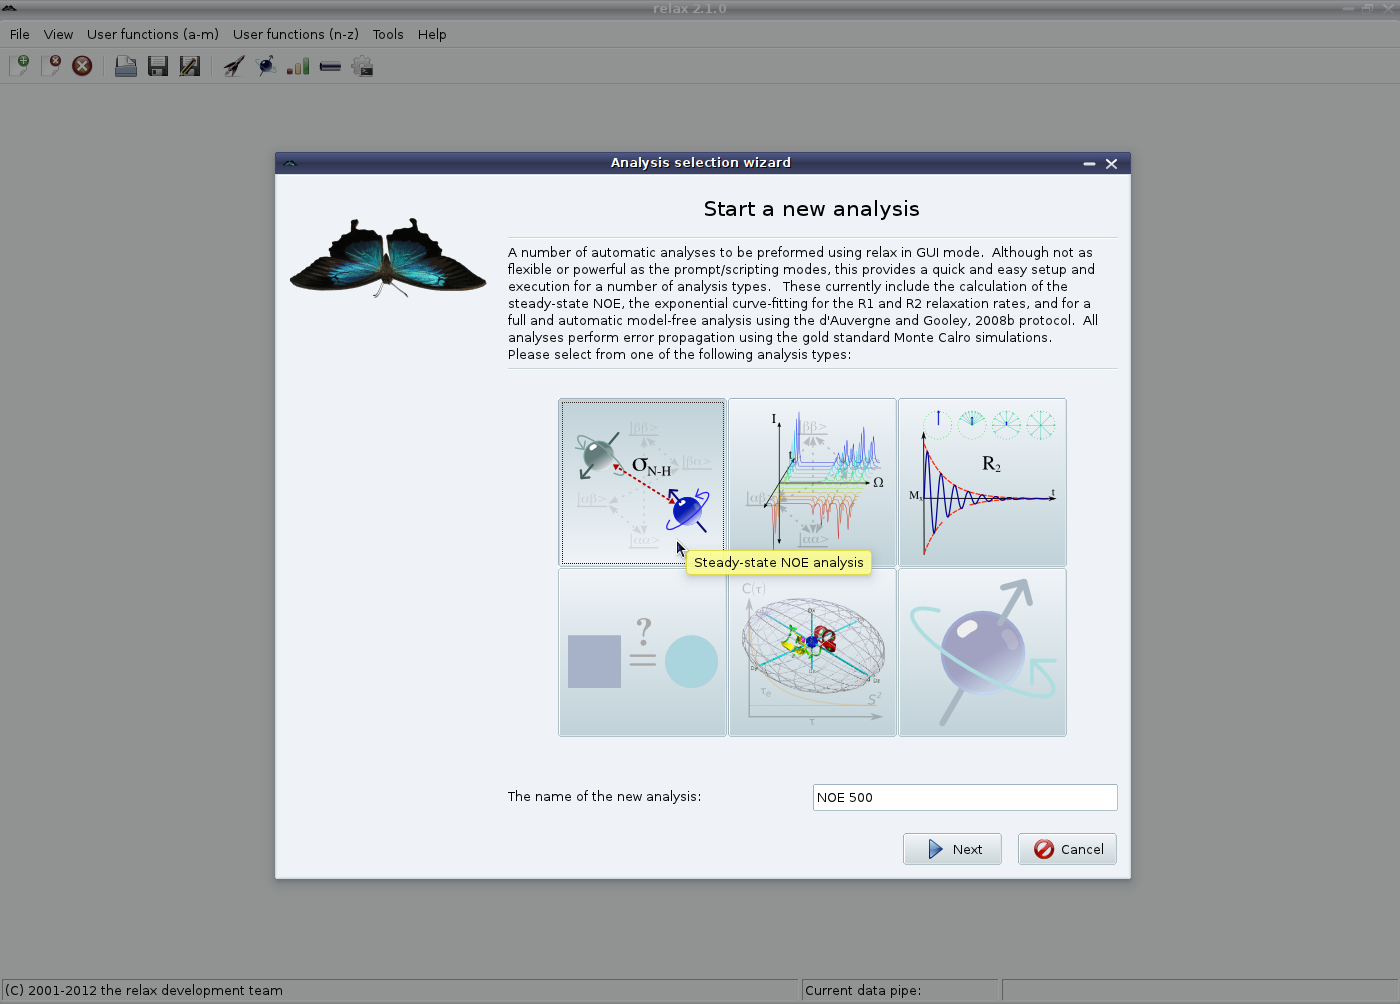
\includegraphics[width=0.8\textwidth, bb=14 14 1415 1019]{graphics/screenshots/noe_analysis/analysis_wizard1}}
\end{minipage}

The second part of the wizard need not be modified, just click on \guibutton{Start} to begin.  This will create a dedicated data pipe for the analysis.  A data pipe bundle will also be created, but for the steady-state NOE will only contain a single data throughout the analysis.

\begin{minipage}[h]{\linewidth}
\centerline{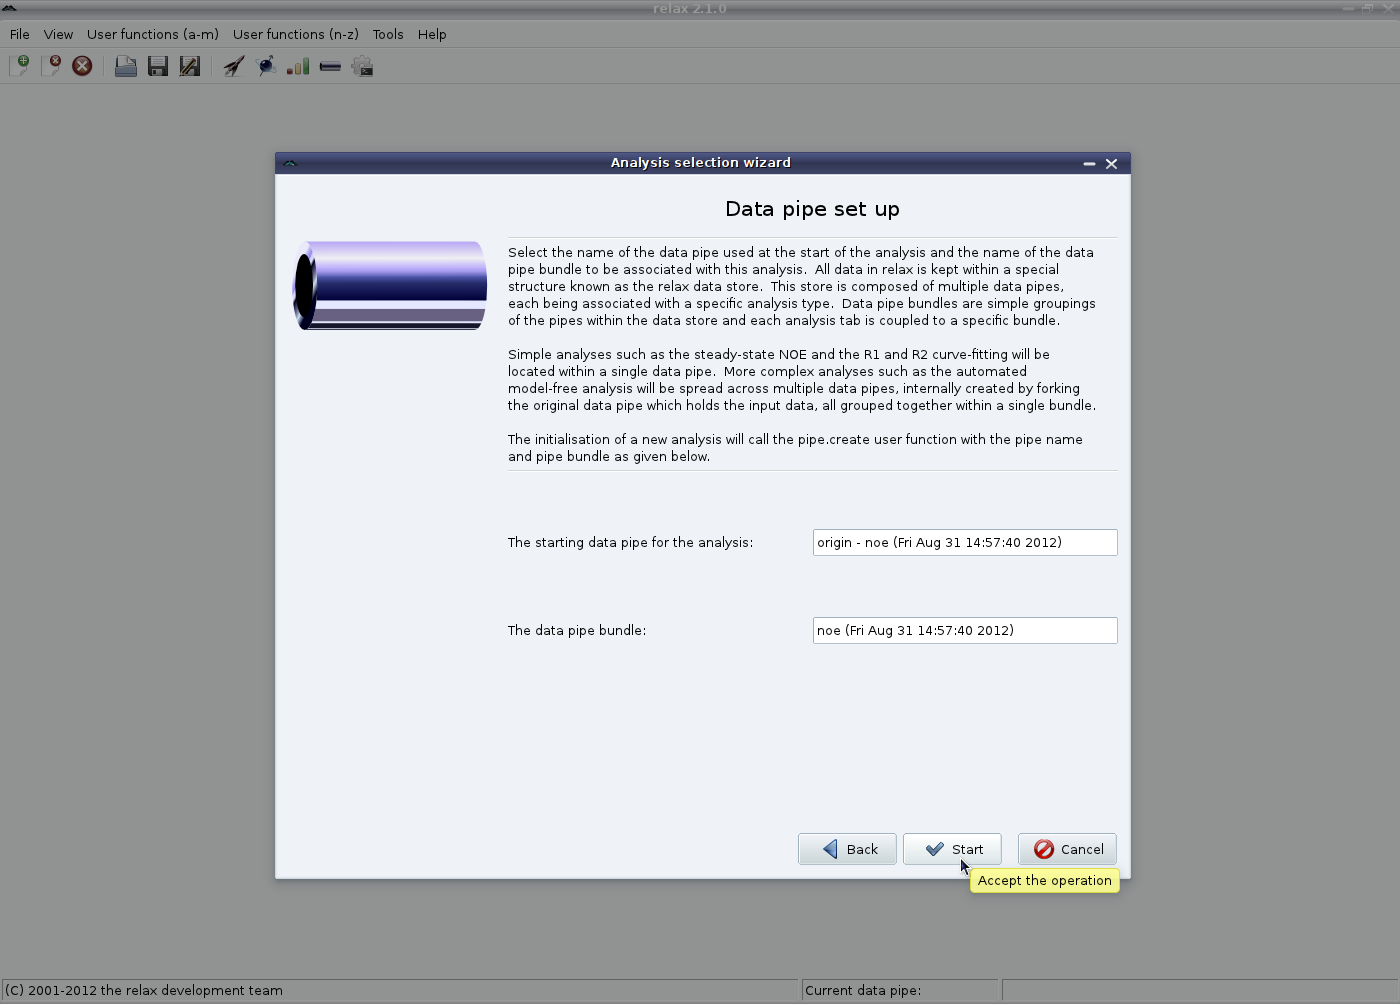
\includegraphics[width=0.8\textwidth, bb=14 14 1415 1019]{graphics/screenshots/noe_analysis/analysis_wizard2}}
\end{minipage}


% General setup.
%~~~~~~~~~~~~~~~

\subsection{NOE GUI mode -- general setup}

You should then see the blank analysis tab:

\begin{minipage}[h]{\linewidth}
\centerline{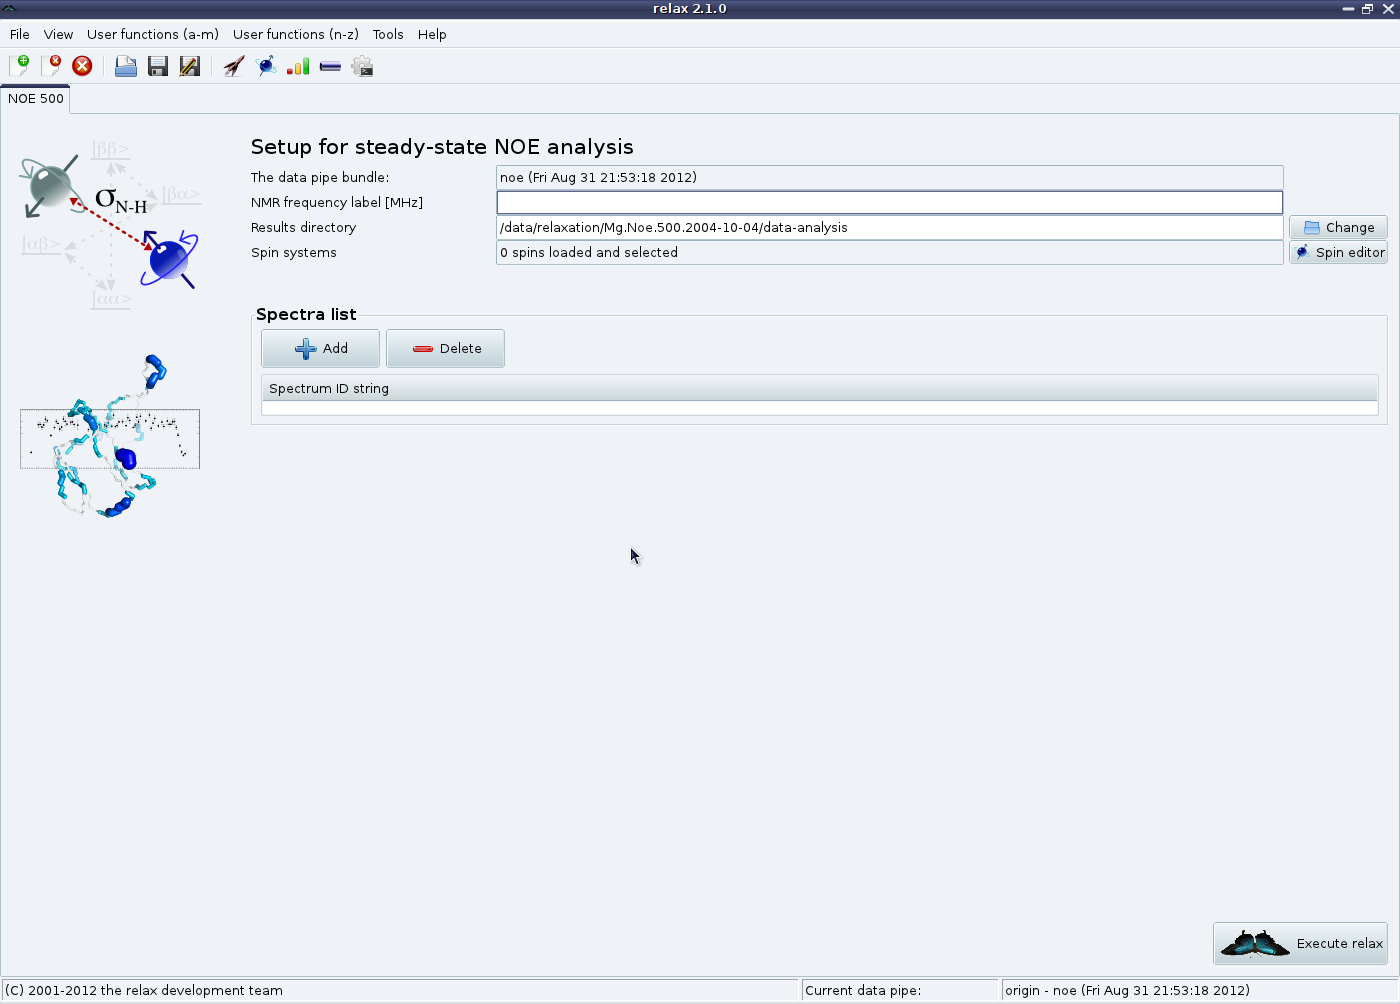
\includegraphics[width=0.8\textwidth, bb=14 14 1415 1019]{graphics/screenshots/noe_analysis/blank}}
\end{minipage}

The first thing to do now is to set the NMR frequency label.  This is only used for the name of the NOE output file.  For example if you set the label to \guistring{500}, the file \file{noe.500.out} will be created at the end of the analysis.

You can also choose to change the \gui{Results directory} where all of the automatically created results files will be placed.  These two steps are unique to the GUI mode.


% Spin systems.
%~~~~~~~~~~~~~~

\subsection{NOE GUI mode -- setting up the spin systems}

Just as in the prompt and scripting UI modes, the molecule, residue and spin data structures need to be set up prior to the loading of any spin specific data.  The \gui{Spin systems} GUI element is used for this purpose.  Before any spin systems have been set up, this should say something like \gui{0 spins loaded and selected}.  To fix this, click on the \guibutton{Spin editor} button and you should then see the spin viewer window.  The next steps are fully described in section~\ref{sect: GUI - structural data} on page~\pageref{sect: GUI - structural data} for PDB files or section~\ref{sect: GUI - sequence file} on page~\pageref{sect: GUI - sequence file} for a sequence file.  The spin viewer window can now be closed.


% Unresolved spins.
%~~~~~~~~~~~~~~~~~~

\subsection{NOE GUI mode -- unresolved spins}

Using the unresolved spins file as described in the prompt/script UI sections, the same spins can be deselected at this point.  See Section~\ref{sect: GUI - deselect spins} on page~\pageref{sect: GUI - deselect spins} for the details of how to deselect the spins in the GUI.


% Loading the data.
%~~~~~~~~~~~~~~~~~~

\subsection{NOE GUI mode -- loading the data}

The next step is to load the saturated and reference NOE peak lists.  From the main NOE auto-analysis tab, click on the \guibutton{Add} button in the \gui{Spectra list} GUI element.  This will launch the NOE peak intensity loading wizard.  From the first wizard page, select the peak list file containing the reference intensities (from the averaged shift list):

\begin{minipage}[h]{\linewidth}
\centerline{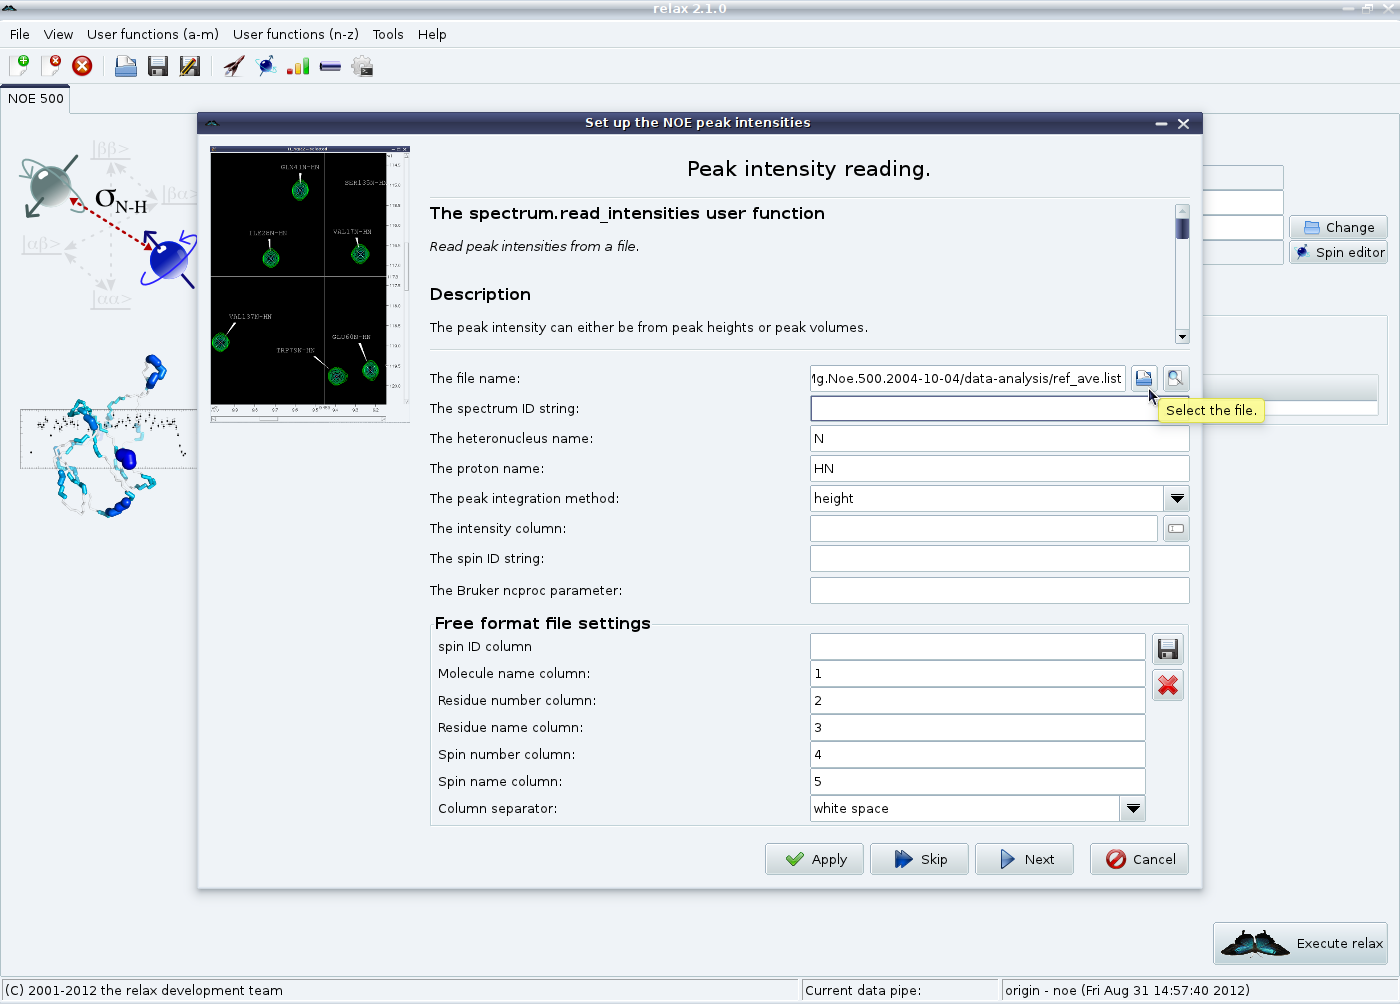
\includegraphics[width=0.8\textwidth, bb=14 14 1415 1019]{graphics/screenshots/noe_analysis/peak_intensity1}}
\end{minipage}

Then set the obligatory spectrum ID string to a unique value (in this case \guistring{ref}).  The heteronucleus and proton names must be changed to match the convention used in the peak list.  In case you have forgotten the spin names, next to the file name selection button is a preview button which can be used to open the peak list in the default text editor.  Set the other fields as needed.

To load the NH data, rather than clicking on \guibutton{Next}, click on \guibutton{Apply}.  This will allow the tryptophan indole data to be loaded in the next step.  Note that a \prompt{RelaxWarning} will be thrown for all peak list entries which do not match the heteronucleus and proton names.  This will cause the relax controller window to appear:

\begin{minipage}[h]{\linewidth}
\centerline{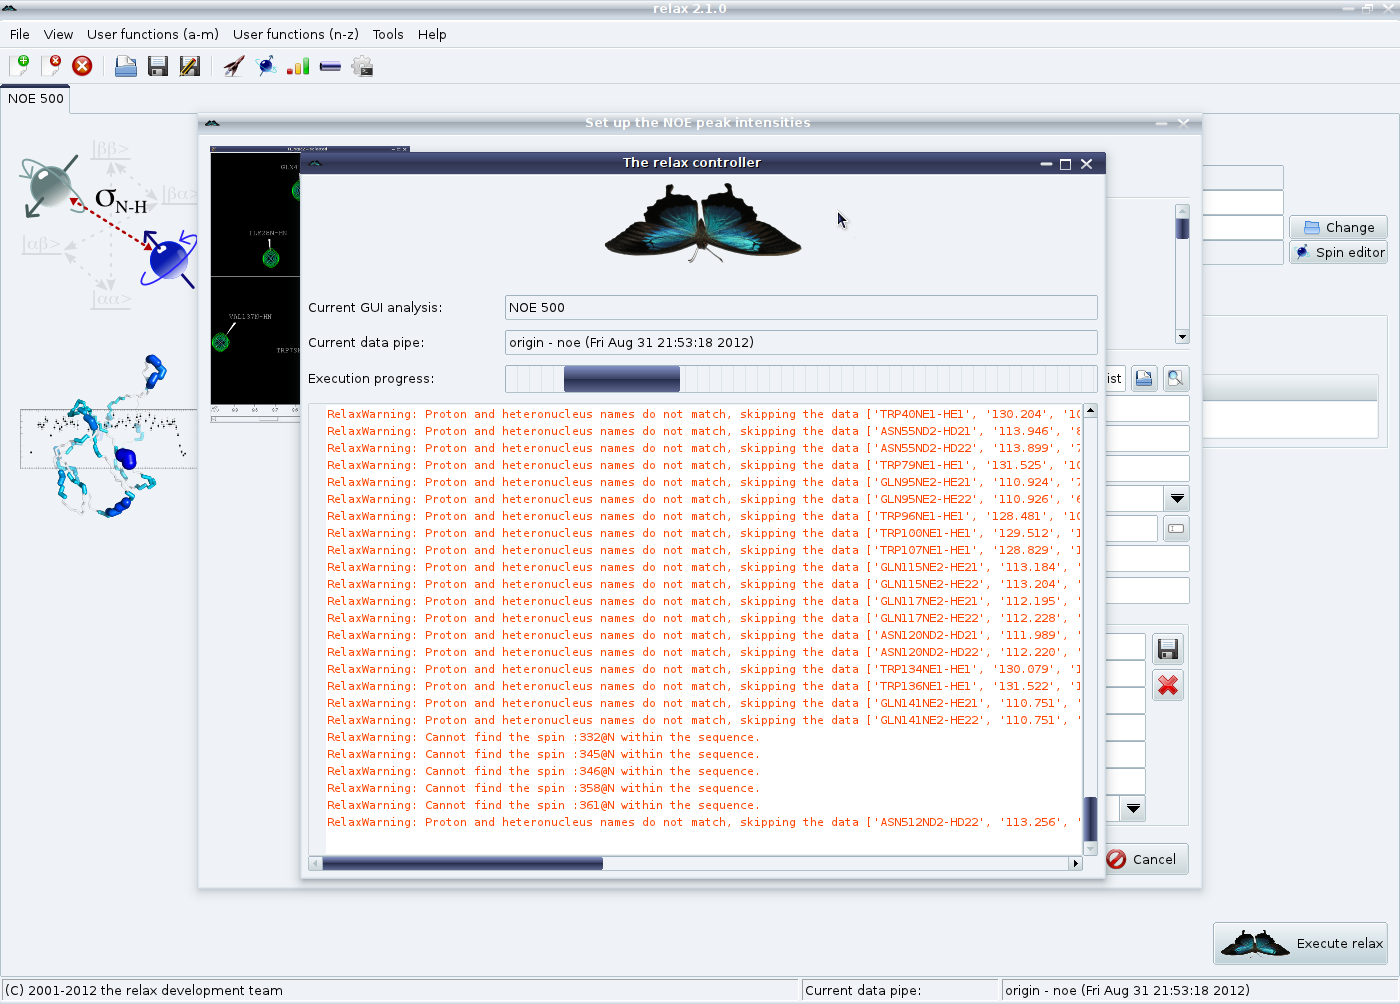
\includegraphics[width=0.8\textwidth, bb=14 14 1415 1019]{graphics/screenshots/noe_analysis/peak_intensity2}}
\end{minipage}

Carefully check these warnings to be sure that the data is correctly loaded, and if everything is fine, the relax controller window can be closed.  If the atom names have been wrongly specified or some other setting is incorrect, a \prompt{RelaxError} might appear saying that no data was loaded -- you will then need to fix the settings and click on \guibutton{Apply} again.  Now change the heteronucleus and protons names to \guistring{NE1} and \guistring{HE1} respectively (or to what ever they have been named in the peak list).  Click on \guibutton{Next}:

\begin{minipage}[h]{\linewidth}
\centerline{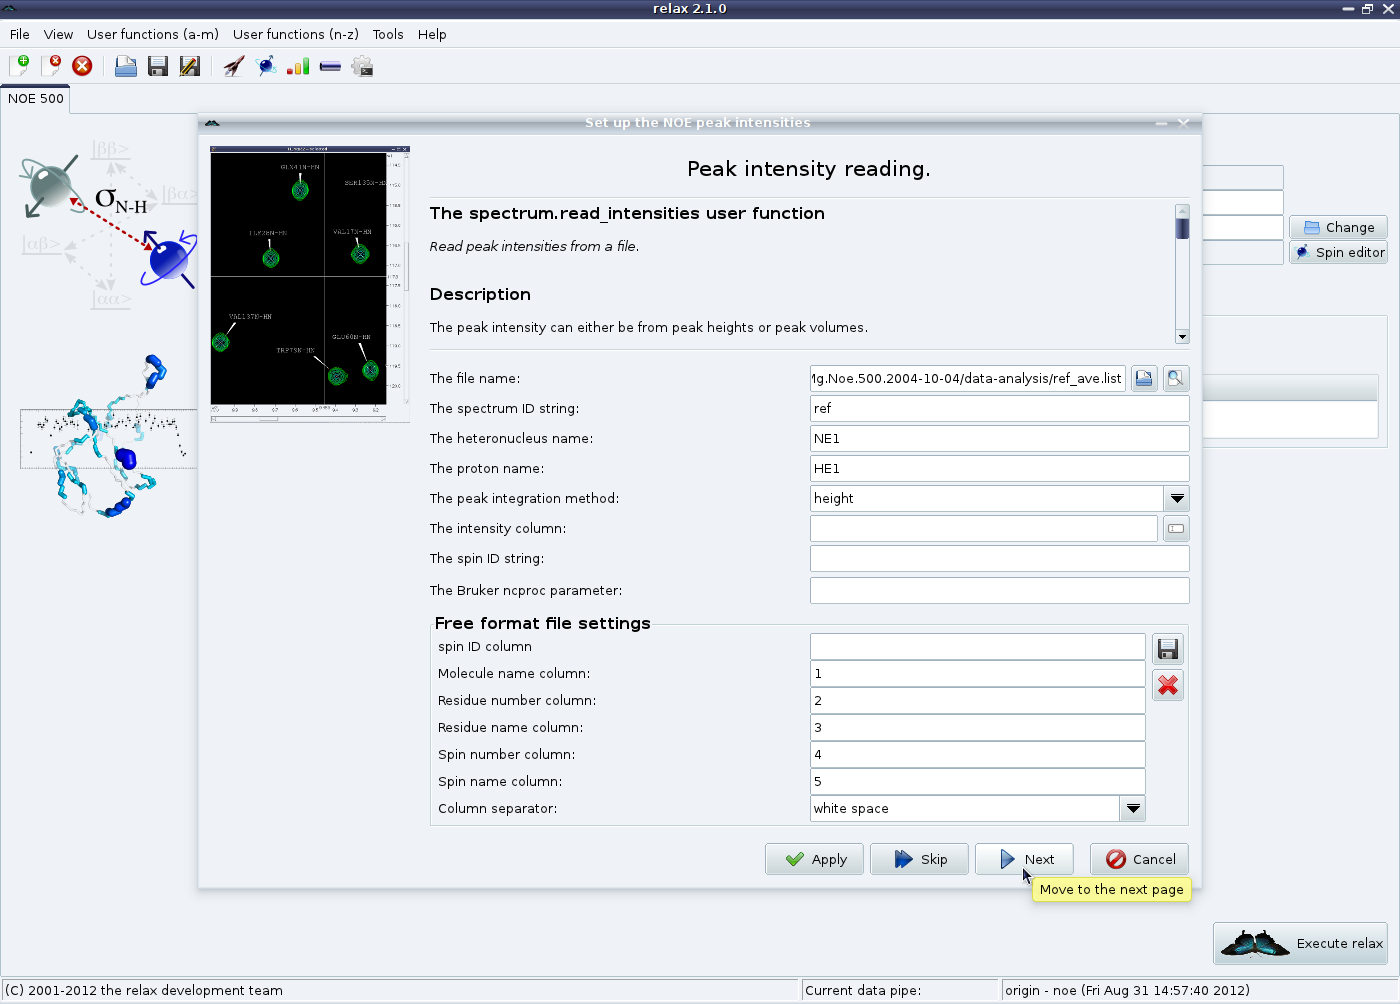
\includegraphics[width=0.8\textwidth, bb=14 14 1415 1019]{graphics/screenshots/noe_analysis/peak_intensity3}}
\end{minipage}

The relax controller will appear again -- check the \prompt{RelaxWarnings} to be sure that the data has loaded correctly then close the controller again.  The error type page should now appear.

\begin{minipage}[h]{\linewidth}
\centerline{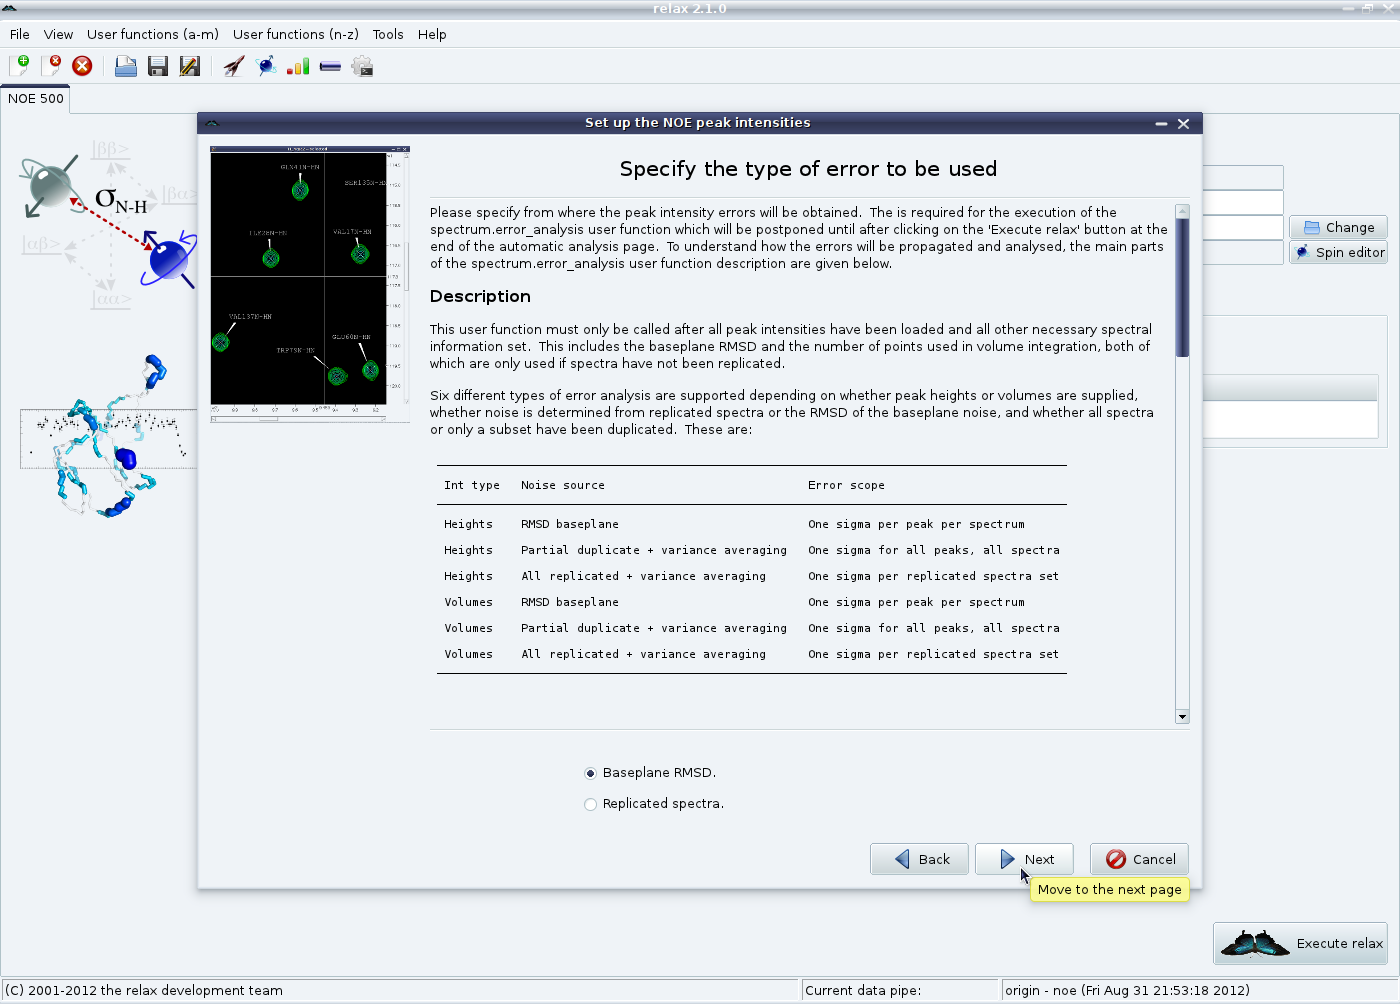
\includegraphics[width=0.8\textwidth, bb=14 14 1415 1019]{graphics/screenshots/noe_analysis/peak_intensity4}}
\end{minipage}

Please read the description in this window very carefully to know what to do next.  In this example, we will choose \gui{Baseplane RMSD}.  For this specific example, Sparky's \guimenuitemthree{Extensions}{Spectrum}{Spectrum baseplane RMSD} option in the \gui{F1} selection mode was used to measure empty regions of the spectrum (mainly in the random coil region) to determine an average RMSD of approximately 3600.  Set the value and click on \guibutton{Apply}.

\begin{minipage}[h]{\linewidth}
\centerline{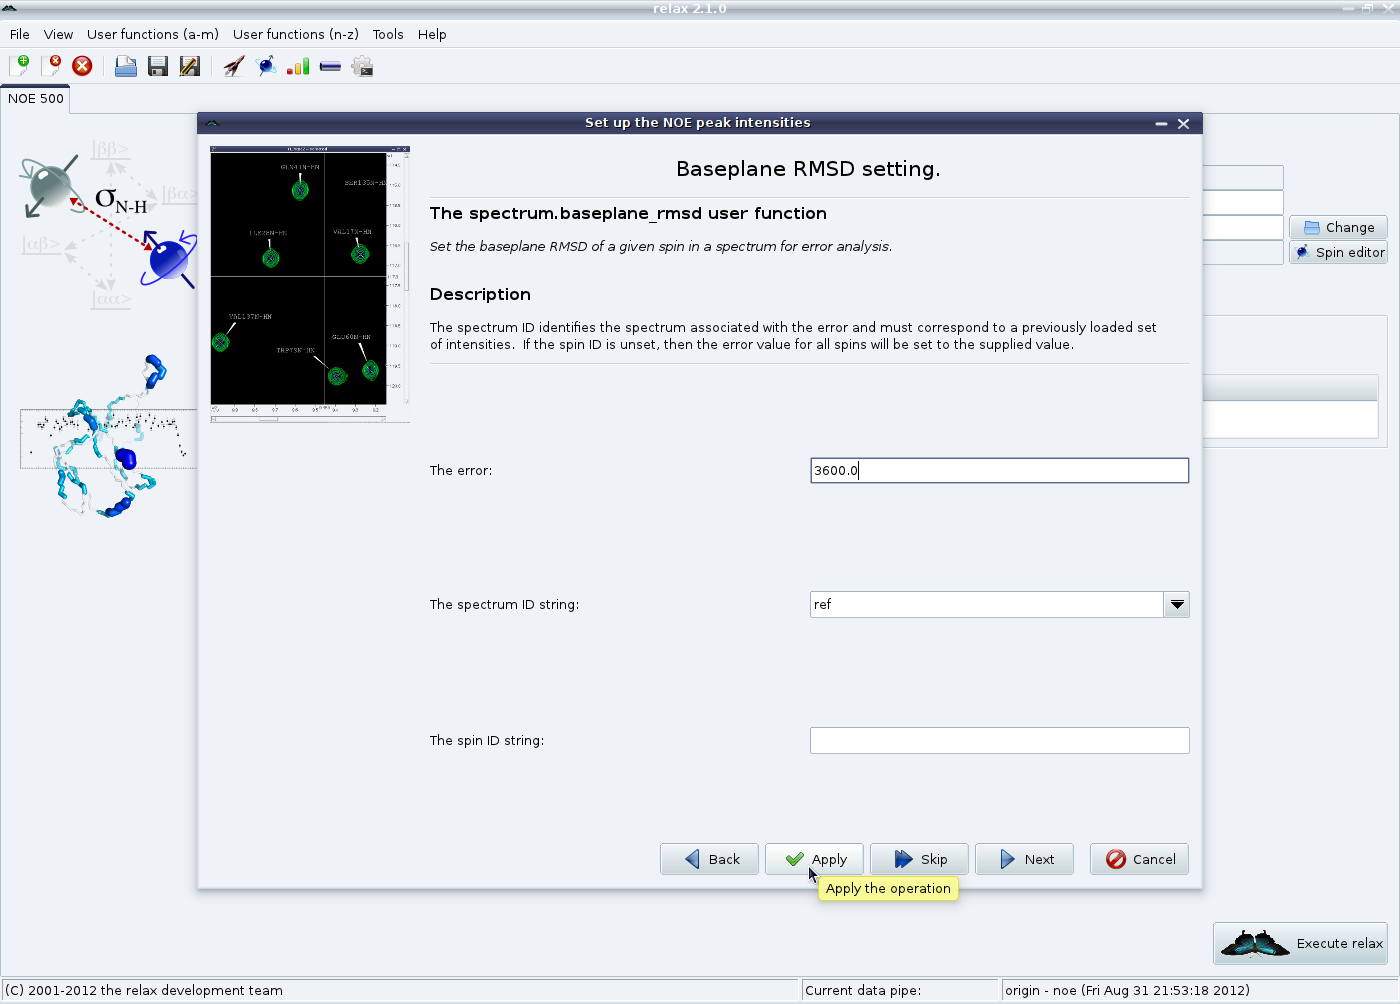
\includegraphics[width=0.8\textwidth, bb=14 14 1415 1019]{graphics/screenshots/noe_analysis/peak_intensity5}}
\end{minipage}

As glycine 114 is located close to the noise signal, its error was much higher at 122000.  Individual spin errors can be set via the spin ID string (see section~\ref{sect: spin ID} on page~\pageref{sect: spin ID} for information about spin IDs):

\begin{minipage}[h]{\linewidth}
\centerline{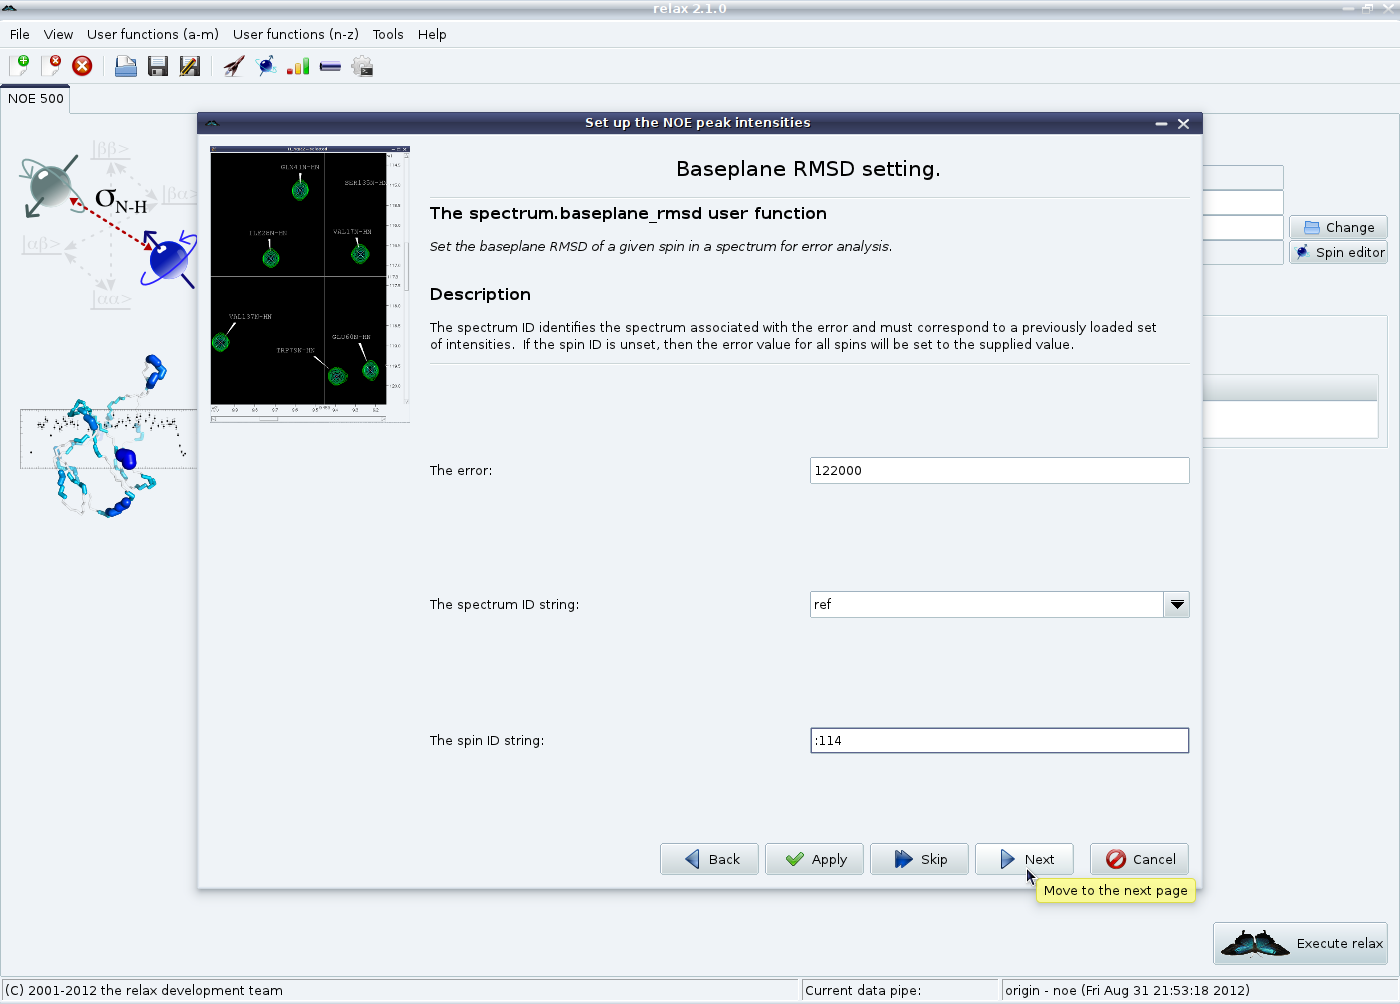
\includegraphics[width=0.8\textwidth, bb=14 14 1415 1019]{graphics/screenshots/noe_analysis/peak_intensity6}}
\end{minipage}

Finally select which type of spectrum this is and click on \guibutton{Finish}:

\begin{minipage}[h]{\linewidth}
\centerline{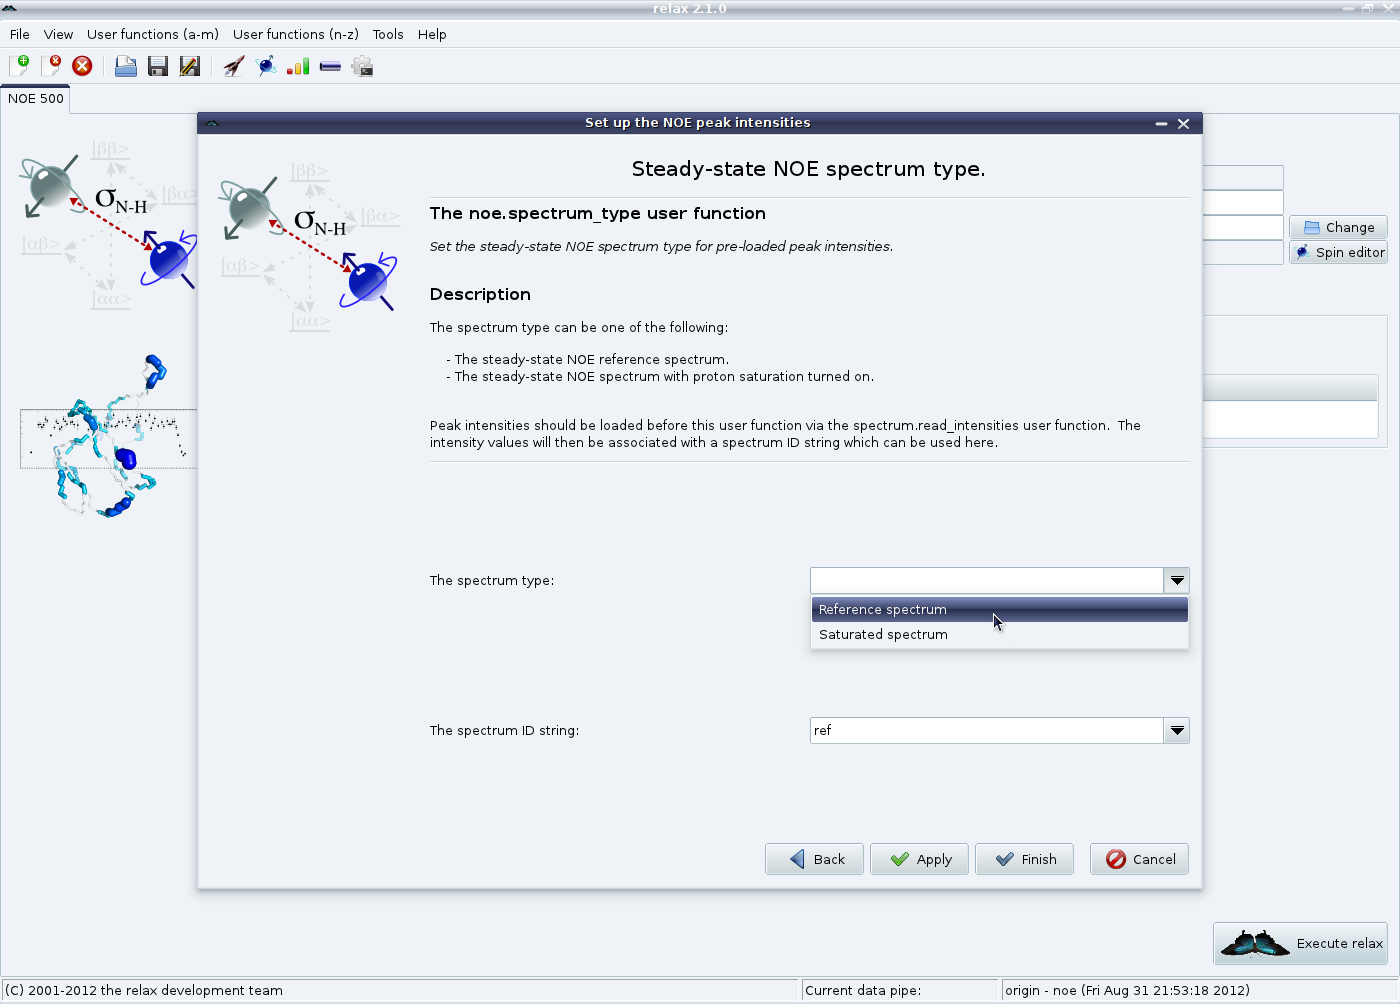
\includegraphics[width=0.8\textwidth, bb=14 14 1415 1019]{graphics/screenshots/noe_analysis/peak_intensity7}}
\end{minipage}

The entire procedure should be repeated for the saturated spectrum (or you may have worked out that both can be loaded simultaneously by using the \guibutton{Apply} button more often).  For this example, the spectrum ID was set to \guistring{sat} and the baseplane RMSD to 3000 for all spins (except for G114 which had an error of 8500).

The NOE analysis tab should now look like:

\begin{minipage}[h]{\linewidth}
\centerline{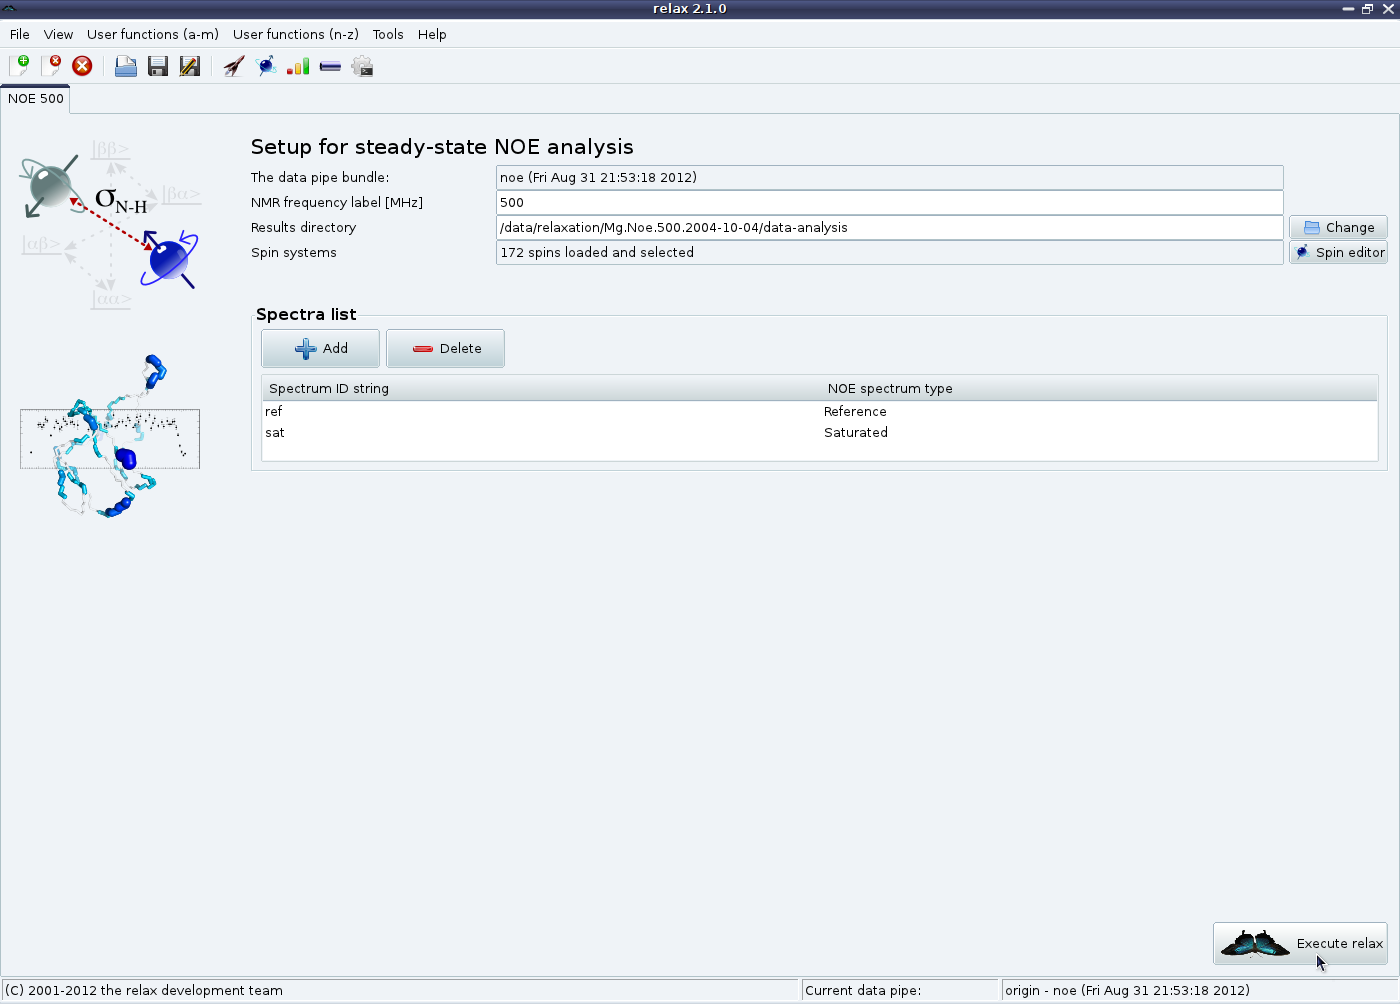
\includegraphics[width=0.8\textwidth, bb=14 14 1415 1019]{graphics/screenshots/noe_analysis/analysis_tab2}}
\end{minipage}


% The NOE.
%~~~~~~~~~

\subsection{NOE GUI mode -- the NOE calculation}

Now that everything is set up, simply click on \guibutton{Execute relax} in the NOE analysis tab.  The relax controller window will appear displaying many messages.  These should all be checked very carefully to make sure that everything has executed as you expected.  The \gui{Results viewer} window will also appear:

\begin{minipage}[h]{\linewidth}
\centerline{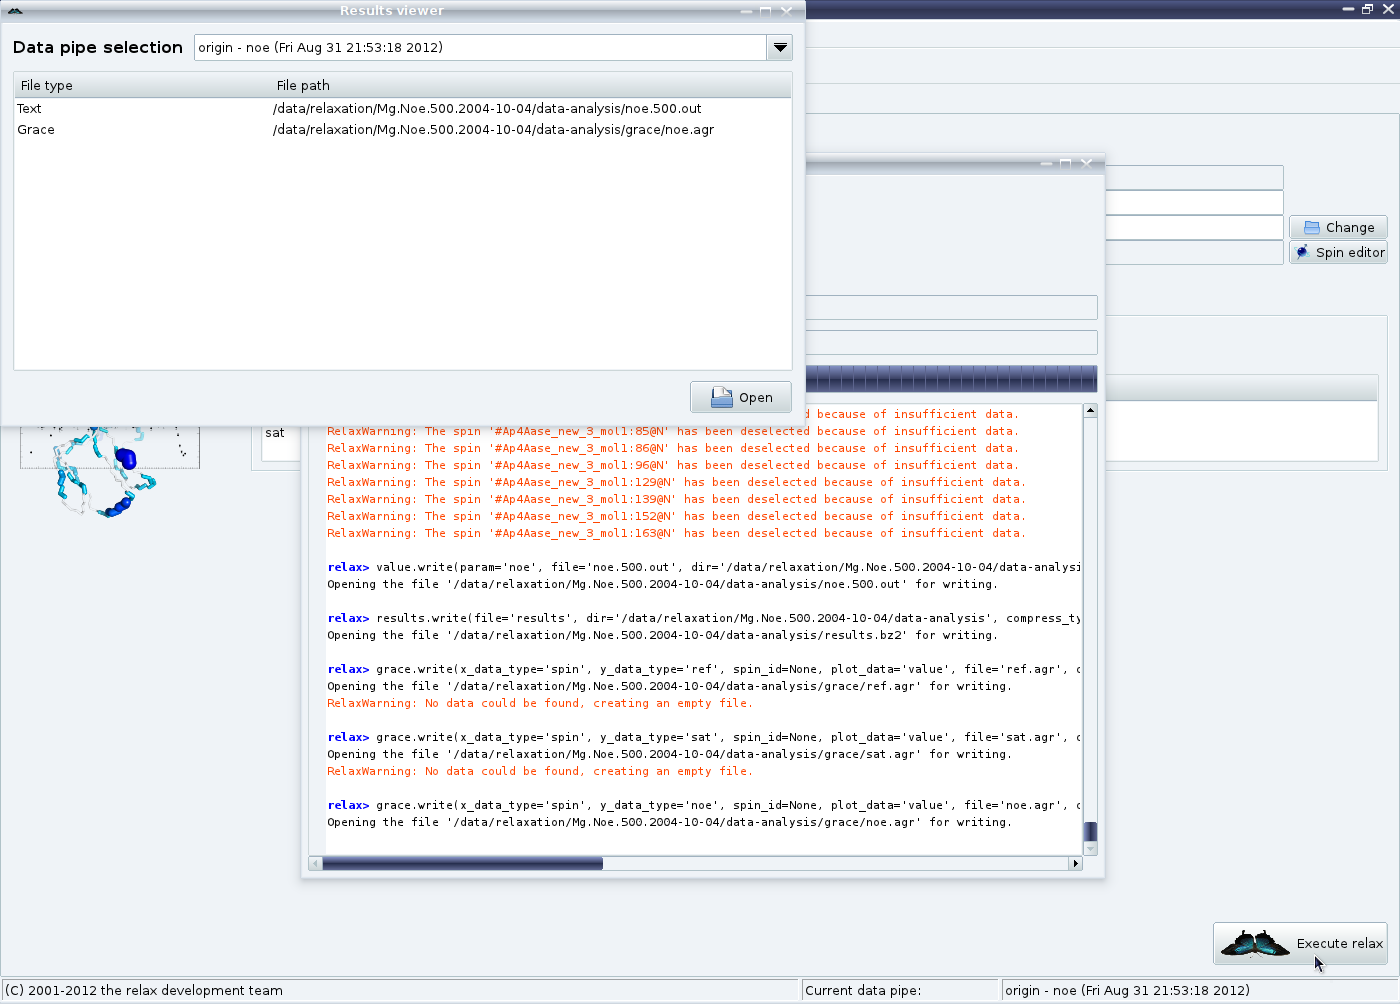
\includegraphics[width=0.8\textwidth, bb=14 14 1415 1019]{graphics/screenshots/noe_analysis/fin}}
\end{minipage}

The results viewer window can be used to launch a text editor to see the NOE values and error or Grace to visualise the results (see Figure~\ref{fig: NOE plot} on page~\pageref{fig: NOE plot}).

As a last step, the relax state can be saved (via the \guimenuitemone{File} menu) and relax closed.  Take one last look at the \file{noe.out} log file to be certain that there are no strange warnings or errors.
